\documentclass[10pt,oneside,slovak,a4paper]{article}

\usepackage[slovak]{babel}

\usepackage[IL2]{fontenc} 
\usepackage[utf8]{inputenc}
\usepackage{graphicx}
\usepackage{listings}
\usepackage{verbatim}
\usepackage{url}
\usepackage{amsfonts}
\usepackage{hyperref} 
\usepackage{cite}
\usepackage[margin=1.3in]{geometry}

\setlength{\tabcolsep}{18pt}
\renewcommand{\arraystretch}{1.5}

\lstset{literate=%
         {á}{{\'a}}1
         {í}{{\'i}}1
         {é}{{\'e}}1
         {ý}{{\'y}}1
         {ú}{{\'u}}1
         {ó}{{\'o}}1
         {ě}{{\v{e}}}1
         {š}{{\v{s}}}1
         {č}{{\v{c}}}1
         {ľ}{{\v{l}}}1
         {ř}{{\v{r}}}1
         {ž}{{\v{z}}}1
         {ď}{{\v{d}}}1
         {ť}{{\v{t}}}1
         {ň}{{\v{n}}}1                
         {ů}{{\r{u}}}1
         {Á}{{\'A}}1
         {Í}{{\'I}}1
         {É}{{\'E}}1
         {Ý}{{\'Y}}1
         {Ú}{{\'U}}1
         {Ó}{{\'O}}1
         {Ě}{{\v{E}}}1
         {Š}{{\v{S}}}1
         {Č}{{\v{C}}}1
         {Ř}{{\v{R}}}1
         {Ž}{{\v{Z}}}1
         {Ď}{{\v{D}}}1
         {Ť}{{\v{T}}}1
         {Ň}{{\v{N}}}1                
         {Ů}{{\r{U}}}1
         {Ä}{{\"A}}1
         {Ľ}{{\v{L}}}1
         {ä}{{\"a}}1    
}

\pagestyle{headings}


\begin{document}

\begin{titlepage}
	\centering
	\par\vspace{1cm}
	{\scshape\LARGE Slovenská technická univerzita v Bratislave \par}
	{\scshape\Large Fakulta informatiky a informačných technológií\par}
	\vspace{1.5cm}
	{\large Princípy informačných systémov \par}
	{\large Dokumentácia projektu\par}
	\vspace{5cm}
	{\huge\bfseries Repozitár - digitálna knižnica\par}
	\vspace{0.5cm}
	{\Large\itshape Dávid Kubík, Martin Staňo, Veronika Včelková\par}
	\vfill
	cvičiaci\par
	RNDr. Marta \textsc{Gnipová}, Ing. Nadežda \textsc{Andrejčíková}, PhD.\par
	\vspace{1cm}
	{\large \today\par}
\end{titlepage}

\tableofcontents

\newpage


\section{Percentuálny podiel práce autov na projekte}

\vspace{1cm}

\begin{tabular}{ |p{3cm}||p{2.5cm}|p{3cm}|p{2.5cm}|}
 \hline
 \multicolumn{4}{|c|}{\textbf{Podiel práce}} \\
 \hline
 Časť projektu & Martin Staňo & Veronika Včelková & Dávid Kubík\\
 \hline
 Počiatočný návrh a identifikácia úloh & 0 & 0 &  0\\
 \hline
 Zapracovanie pripomienok z konzultácií a vytvorenie návrhu v IBM BPM & 0 & 0 &  0\\
 \hline
 Návrh formulárov & 0 & 0 &  0\\
 \hline
 Návrh použitia webových služieb & 0 & 0 &  0\\
 \hline
 Implementácia v IBM BPM & 0 & 0 &  0\\
 \hline
 Vypracovanie dokumentácie & 0 & 0 &  0\\
 
 \hline
\end{tabular}

\newpage

\section{Špecifikácia projektu: Repozitár - digitálna knižnica}

\subsection{Úvod}

Cieľom tohto projektu je definovať biznis procesy na podporu nižšie popísanej problémovej domény. Tieto biznis procesy budu navrhnuté, implementované a otestované v prostredí IBM BPM. Pri návrhu a implementácií biznis procesov sa dbalo na dodržiavanie princípov SOA (využívanie webových služieb a ich správne prepojenie).


\subsection{Zadanie - špecifikácia}

Horizont H2020 určuje vedeckovýskumným pracoviskám povinnosť evidovať svoje publikované výsledky VaV v repozitári – vlastnom, konzorcionálnom, národnom. Údaje, ktoré popisujú dokument – bibliografický záznam, môže vykonávať spracovateľ, knihovník, alebo priamo vedec.

Formulár obsahuje minimálne všetky základné údaje nevyhnutné pre jednoznačnú identifikáciu daného typu dokumentu. Pri vkladaní dát sú priebežne systémom vykonávané viaceré kontroly, dôležité je, aby všetky entity boli identifikovaný perzistentným jedno-jednoznačným identifikátorom, teda aby v systéme nemohli na základe termínu reprezentujúceho dané idivídum vznikať homonymá, ale zároveň aby systém vedel k danému termínu agregovať všetky jeho synonymá, akronymy, či iné variantné formy termínov, ktoré môžu vystihovať význam tohto indivídua.

Zadané údaje sa vždy uložia do systému aj s prípadnými chybami, všetky údaje sú logované a v prípade, že neexistuje identifikátor pre dané indivídum entity, systém vytvorí nový záznam pre toto individum a pridelí mu požadovaný identifikátor a následne vo formulári prelinkuje na tento identifikátor.

Všetky vzťahy medzi entitami sú evidované na základe významu a prostredníctvom uvedených identifikátorov, teda nie odkaz na termín, ten sa generuje následne prostredníctvom daného identifikátora z príslušnej databázy modelu. 

Konečnú platnosť a správnosť údajov, môže potvrdiť až knihovník, vtedy sa všetky údaje pre iný používateľov a teda aj autorov stávajú len read/only, návrh na akúkoľvek zmenu môžu vykonať len prostredníctvom mailu, alebo poznámky k záznamu. Ak údaje vkladá spracovateľ, alebo vedecký pracovník, ostatní spoluautori ako aj konkrétny spracovateľ sú o tom informovaní , rovnako ako aj v prípade, keď knihovník potvrdí správnosť a zverejní záznam. 

Samozrejme autori určujú podmienky, pre koho bude záznam aj dokument dostupný voľne a pre ktoré skupiny na vyžiadanie, prípadne pre koho zasa úplne neviditeľný, pričom môže toto kombinovať aj s časovým určením, teda napr. pre pracovníkov oddelenia voľne dostupný pre ostatných akademických a vedecko-pedagogických pracovníkov voľne dostupný po 2 rokoch a pre ostatných viditeľný po 3 a voľne dostupný po 5 rokoch.

Navrhnite procesy, ktoré umožnia spracovať a sprístupňovať repozitár publikovaných výsledkov vedy a výskumu tak, že bude zároveň evidovať všetky vzájomné vzťahy medzi entitami použitými pre popis publikovaného výsledku VaV na základe významu.

\newpage

\section{Návrh, analýza a opis biznis procesov}

V tomto projekte budú analyzované a implementované nasledujúce biznis procesy súvisiace s problémovou doménou:

\begin{itemize}
\item Nahranie bibliografického záznamu
\item Aktualizácia bibliografického záznamu
\item Vyhľadanie bibliografického záznamu
\end{itemize}

\subsection{Dátový model}

Vo vyššie pomenovaných biznis procesoch sme identifikovali nasledujúce entity ako aj ich atribúty a vzťahy medzi nimi. Tieto entity zároveň reprezentujú naše biznis objekty (komplexné dátové typy).

\begin{figure}[h]
\label{datamodel}
\centering
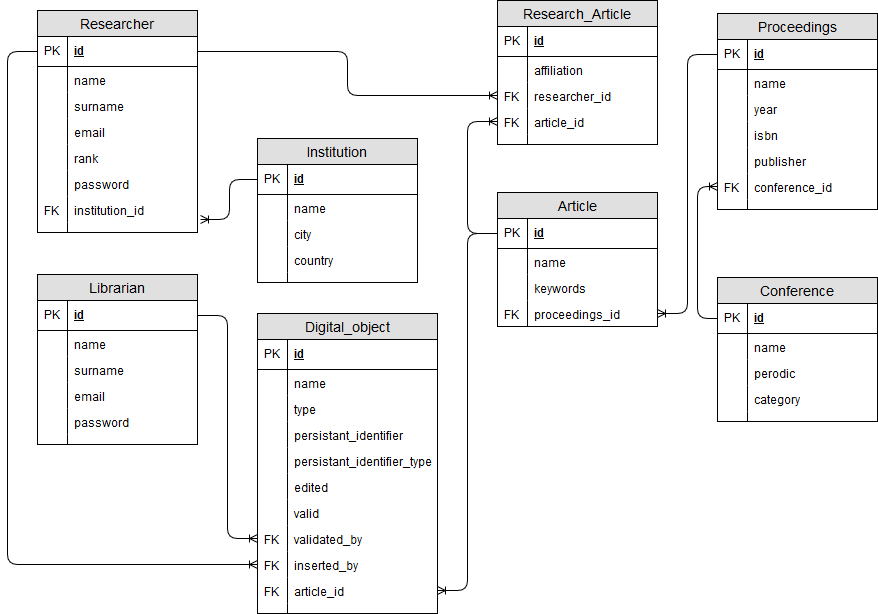
\includegraphics[scale=0.4]{datovy_model.png} 
\caption{ER diagram dátového modelu}
\end{figure}

\subsection{Nahranie bibliografického záznamu}
V nasledujúcich podkapitolách sa bližšie pozrieme na biznis proces - nahranie bibliografického záznamu.

\subsection{Cieľ biznis procesu}
Cieľom tohto biznis procesu je nahranie bibliografického záznamu do konkrétneho digitálneho repozitára. Knihovník vykoná kontrolu údajov a potvrdí ich potencionálnu správnosť.

\subsection{Používateľské roly}
Jednotlivé kroky procesu sú rozdelené do troch plaveckých dráh.

\begin{itemize}
\item \textbf{Systém} Táto plavecká dráha obsahuje úlohy, ktoré bude vykonávať nami navrhovaný systém.
\item \textbf{Používateľ} Táto plavecká dráha obsahuje úlohy, ktoré bude vykonávať používateľ systému. Používateľom, môže byť spracovateľ, knihovník, alebo vedec.
\item \textbf{Knihovník} Táto plavecká dráha obsahuje úlohy, ktoré bude vykonávať knihovník.
\end{itemize}

\subsection{Biznis objekty}
\textbf{Institucia}\\
Tento biznis objekt reprezentuje vedeckovýskumné pracovisko, ktoré eviduje publikované výsledky v repozitári. Parametre tohto biznis objektu sú nasledovné:

\begin{itemize}
\item \textbf{id:} unikátny primárny kľúč v systémovej databáze,
\item \textbf{name:} názov inštitúcie, pod ktorým je registrovaná v obchodnom registri Slovenskej republiky,
\item \textbf{city:} mesto, v ktorom má daná inštitúcia hlavné sídlo,
\item \textbf{country:} krajina, v ktorom je hlavné sídlo danej inštitúcie.
\end{itemize}

\textbf{Knihovnik}\\
Tento biznis objekt reprezentuje zamestnanca vedeckovýskumného pracoviska, ktorý má na starosti okrem iného aj potvrdzovanie správnosti zadaných údajov bibliografického záznamu. Parametre tohto biznis objektu sú nasledovné:

\begin{itemize}
\item \textbf{id:} unikátny primárny kľúč v systémovej databáze,
\item \textbf{name:} krstné meno uvedené v rodnom liste pracovníka vedeckovýskumného ústavu,
\item \textbf{last\_name:} priezvisko uvedené v rodnom liste pracovníka vedeckovýskumného ústavu,
\item \textbf{email:} emailová schránka pracovníka vedeckovýskumného ústavu,
\item \textbf{institucia\_id:} cudzí kľúč v systémovej databáze, ktorý sa odkazuje na konkrétnu inštitúciu,
\item \textbf{rank:} úroveň pracovníka k sprístupneniu publikácií.
\end{itemize}

\textbf{Vedec}\\
Tento biznis objekt reprezentuje zamestnanca vedeckovýskumného pracoviska, ktorý svoje výsledky publikuje do digitálneho repozitára. Parametre tohto biznis objektu sú nasledovné:

\begin{itemize}
\item \textbf{id:} unikátny primárny kľúč v systémovej databáze,
\item \textbf{name:} krstné meno uvedené v rodnom liste pracovníka vedeckovýskumného ústavu,
\item \textbf{last\_name:} priezvisko uvedené v rodnom liste pracovníka vedeckovýskumného ústavu,
\item \textbf{email:} emailová schránka pracovníka vedeckovýskumného ústavu,
\item \textbf{institucia\_id:} cudzí kľúč v systémovej databáze, ktorý sa odkazuje na konkrétnu inštitúciu,
\item \textbf{rank:} úroveň pracovníka k sprístupneniu publikácií.
\end{itemize}

\textbf{Vedec\_Publikacia}\\
Tento biznis objekt reprezentuje prepojovaciu tabuľku v systémovej databáze medzi vedcami a publikáciami. K tomuto kroku sme pristúpili z dôvodu, aby sme vedeli korektne vyjadriť vzťah many-to-many. Parametre tohto biznis objektu sú nasledovné:

\begin{itemize}
\item \textbf{id:} unikátny primárny kľúč v systémovej databáze,
\item \textbf{vedec\_id:} cudzí kľúč v systémovej databáze, ktorý sa odkazuje na autora publikovaného bibliografického záznamu v digitálnom repozitári,
\item \textbf{publikacia\_id:} cudzí kľúč v systémovej databáze, ktorý sa odkazuje na publikovaný bibliografický záznam v digitálnom repozitári.
\end{itemize}

\textbf{Publikacia}\\
Tento biznis objekt reprezentuje bibliografický záznam v databáze vedeckovýskumného pracoviska. Parametre tohto biznis objektu sú nasledovné:

\begin{itemize}
\item \textbf{id:} unikátny primárny kľúč v systémovej databáze,
\item \textbf{name:} názov publikácie, pod ktorým je uvedená v databáze vedeckovýskumného pracoviska,
\item \textbf{isbn:} medzinárodné štandardné číslo knihy (z angl. international standard book number) pod ktorým bol bibliografický záznam publikovaný,
\item \textbf{keywords:} kľúčové slová, ktoré sa využívajú pri vyhľadaní danej publikácie v digitálnom repozitári,
\item \textbf{abstrakt\_text:} stručný výťah publikovaného bibliografického záznamu,
\item \textbf{published\_date:} dátum, kedy bol daný bibliografický záznam publikovaný v zborníku,
\item \textbf{reviewed\_date:} dátum, kedy bola publikácia revidovaná. 
\end{itemize}

\textbf{Repozitar}\\
Tento biznis objekt reprezentuje digitálny repozitár. Parametre tohto biznis objektu sú nasledovné:

\begin{itemize}
\item \textbf{id:} unikátny primárny kľúč v systémovej databáze,
\item \textbf{name:} názov digitálneho repozitáru,
\item \textbf{druh\_id} cudzí kľúč v systémovej databáze, ktorý sa odkazuje na konkrétny typ digitálneho repozitáru.
\end{itemize}

\textbf{Druh}\\
Tento biznis objekt reprezentuje typ digitálneho repozitáru. Digitálny repozitár môže byť napríklad vlastný, konzorcionálny alebo národný. Parametre tohto biznis objektu sú nasledovné:

\begin{itemize}
\item \textbf{id:} unikátny primárny kľúč v systémovej databáze,
\item \textbf{name:} typ digitálneho repozitáru.
\end{itemize}

\textbf{Notifikacia}\\
Tento biznis objekt reprezentuje notifikácie, ktoré informujú spoluautorov a konkrétneho spracovateľa o vložení údajov ako aj informujú o potvrdení správnosti týchto údajov knihovníkom a informujú tiež o zverejnení publikácie. Parametre tohto biznis objektu sú nasledovné:

\begin{itemize}
\item \textbf{id:} unikátny primárny kľúč v systémovej databáze,
\item \textbf{subject:} hlavička (predmet) notifikácie,
\item \textbf{knihovnik\_id:} cudzí kľúč v systémovej databáze, ktorý sa odkazuje na konkrétneho knihovníka vedeckovýskumného ústavu, ktorého akcia vyvolala vygenerovanie notifikácie,
\item \textbf{vedec\_id:} cudzí kľúč v systémovej databáze, ktorý sa odkazuje na konkrétneho vedca vedeckovýskumného ústavu, ktorý je adresátom notifikácie,
\item \textbf{notification\_text:} Obsah notifikácie obsahujúci podrobnejšie informácie,
\item \textbf{type:} typ notifikácie,
\item \textbf{sent\_date:} dátum odoslania notifikácie.
\end{itemize}

\textbf{Pripomienka}\\
Tento biznis objekt reprezentuje pripomienku na zmenu údajov už publikovaného bibliografického záznamu, ktorého údaje boli zároveň skontrolované a ich správnosť potvrdená knihovníkom. Parametre tohto biznis objektu sú nasledovné:

\begin{itemize}
\item \textbf{id:} unikátny primárny kľúč v systémovej databáze,
\item \textbf{submitted\_by:} krstné meno a priezvisko vedca vedeckovýskumného pracoviska, ktorý navrhuje úpravu údajov v bibliografickom zázname,
\item \textbf{zaznam\_id:} 
\item \textbf{subject:} hlavička (predmet) pripomienky,
\item \textbf{comment\_text:} Obsah pripomienky obsahujúci podrobnejšie informácie o zmenách, ktoré chce vedec vykonať v bibliografickom zázname,
\item \textbf{submited\_date:} dátum podania pripomienky,
\item \textbf{commited:} pravdivostná hodnota, či knihovník zapracoval úpravy údajov v publikovanom bibliografickom zázname.
\end{itemize}

\textbf{Zaznam}\\
Tento biznis objekt reprezentuje publikovaný bibliografický záznam v digitálnom repozitári. Parametre tohto biznis objektu sú nasledovné:

\begin{itemize}
\item \textbf{id:} unikátny primárny kľúč v systémovej databáze,
\item \textbf{name:} názov publikácie, pod ktorým je uvedená v digitálnom repozitári,
\item \textbf{valid:} pravdivostná hodnota, ktorá vyjadruje, či sú údaje v publikácii správne,
\item \textbf{edited:} dátum, kedy bola publikácia v digitálnom repozitári naposledy upravená,
\item \textbf{validated:} dátum, kedy bolo rozhodnuté, že údaje v publikácii sú validné,
\item \textbf{accessible\_by:} vyjadruje minimálnu požadovanú úroveň pracovníka k sprístupneniu publikácie,
\item \textbf{knihovnik\_id:} cudzí kľúč v systémovej databáze, ktorý sa odkazuje na konkrétneho knihovníka,
\item \textbf{vedec\_id:} cudzí kľúč v systémovej databáze, ktorý sa odkazuje na konkrétneho vedca,
\item \textbf{repozitar\_id:} cudzí kľúč v systémovej databáze, ktorý sa odkazuje na konkrétny repozitár.

\end{itemize}

\section{Zhrnutie}
TODO

\section{Report práce členov tímu}




\end{document}